\chapter{Modelo de estados}
A continucación describiremos de manera detallada el modelo de estados correspondiente a las entidades de vacantes, postulaciones, reclutadores
y empresas.
\section{Máquina de estados de una vacante}
\subsection{Resumen}
En todo momento una vacante tiene un ``estado'' en el sistema. Las acciones que
los actores pueden realizar sobre dicha vacante dependen del estado y pueden tener como
consecuencia la transición a otro estado.
Los estados y transiciones posibles se muestran en la
figura  y se describen a continuación.
\begin{figure}[hbtp!]
    \begin{center}
        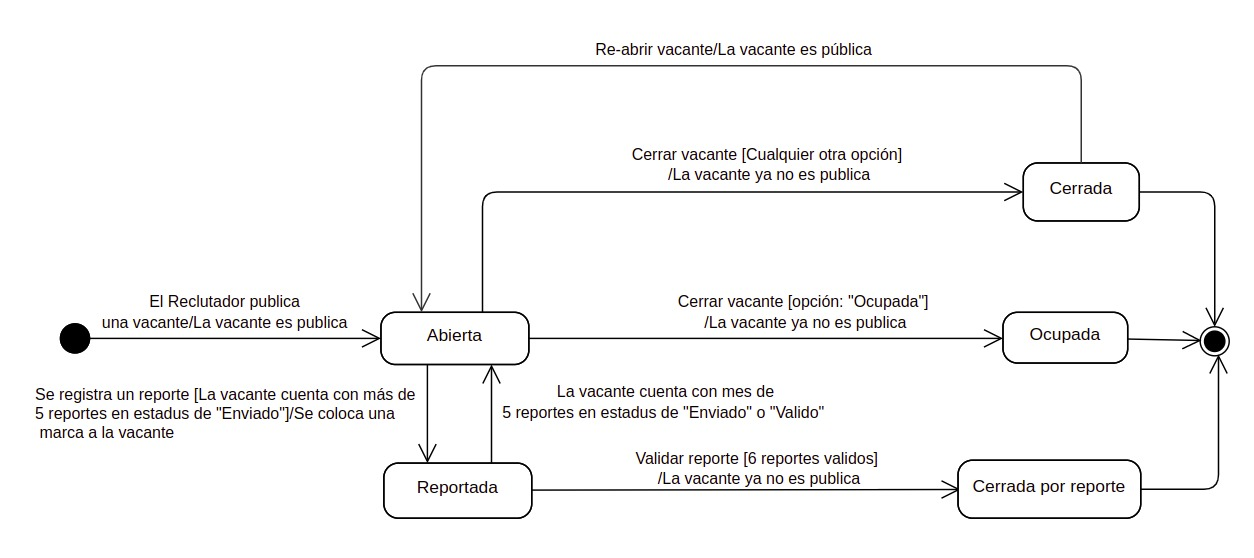
\includegraphics[width=.6\textwidth]{anexos/imagenes/mvacante.jpeg}
    \end{center}
    \caption{Máquina de estados de una vacante.}
    \label{fig:arquitectura}
\end{figure}


\subsection{Descripción}

La tabla \ref{figvacante} muestra el comportamiento que se tendrá en los íconos de la pantalla 
\refElem{VCT-IU08}, los cuales son habilitados dependiendo del estado en el que se encuentre  la vacante.


\begin{table}[htbp]
	\begin{center}
		\begin{tabular}{|c|c|c|c|}
			\hline
			Estado &\IUbutton{Cerrar vacante}& \IUEliminar & \IUEditar \\
			\hline \hline
			Abierta  & Habilitado & Habilitado & Habilitado \\ \hline
			Cerrada & No aparece & Habilitado & Habilitado \\ \hline
			Ocupada & Habilitado & Habilitado & No aparece \\ \hline
			Reportada & No aparece & Habilitado & Habilitado \\ \hline
            Cerrada por reporte & No aparece & Habilitado & Habilitado\\ \hline
		\end{tabular}
		\caption{Comportamiento de acciones para gestionar vacantes.} \label{PLA-CAT-AccionesAnteproyecto}

	\end{center}
\end{table}


\section{Máquina de estados de una postulación}
\subsection{Resumen}
En todo momento una postulación tiene un ``estado'' en el sistema. Las acciones que
los actores pueden realizar sobre dicha postulación dependen del estado y pueden tener como
consecuencia la transición a otro estado.
Los estados y transiciones posibles se muestran en la
figura  y se describen a continuación.
\begin{figure}[hbtp!]
    \begin{center}
        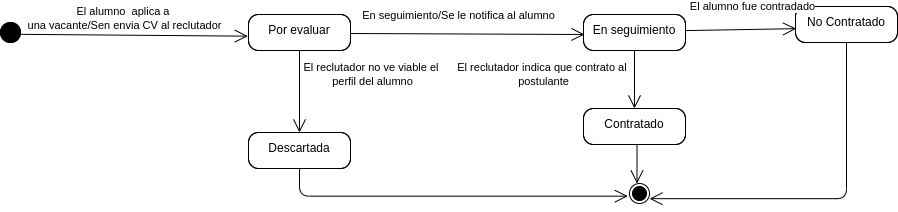
\includegraphics[width=.6\textwidth]{anexos/imagenes/mpost.png}
    \end{center}
    \caption{Máquina de estados de una postulación}
    \label{fig:arquitectura}
\end{figure}


\subsection{Descripción}

La tabla \ref{figvacante} muestra el comportamiento que se tendrá en los íconos de la pantalla 
\refElem{VCT-IU08}, los cuales son habilitados dependiendo del estado en el que se encuentre  la vacante.


\begin{table}[htbp]
	\begin{center}
		\begin{tabular}{|c|c|c|c|c|}
			\hline
			Estado &\IUbutton{Seguimiento}& \IUbutton{Descartar} & \IUbutton{Contratado} & \IUbutton{No Contratado}\\
			\hline \hline
			Por evaluar  & Habilitado & Habilitado & No aparece & No aparece\\ \hline
			Descartada & No aparece & No aparece & No aparece & No aparece\\ \hline
			En seguimiento & No aparece & No aparece & Habilitado & Habilitado\\ \hline
			Contratado & No aparece & No aparece & No aparece & No aparece\\ \hline
            No contratado & No aparece & No aparece & No aparece & No aparece\\ \hline
		\end{tabular}
		\caption{Comportamiento de acciones para gestionar postulaciones.} \label{PLA-CAT-AccionesAnteproyecto}

	\end{center}
\end{table}

